\chapter{Trees}

\section{Properties of Trees}

\begin{definition}[Forests]
  A \textit{forest} is a graph that contains no cycle. Note that the graph 
  does not have to be connected to be a forest.
\end{definition}

\begin{definition}[Trees]
  A \textit{tree} is a connected graph with no cycle.
\end{definition}

\begin{theorem}
  A graph \(G\) is a tree if and only if every two vertices in \(G\) are
  connected by a unique path.
\end{theorem}

\begin{proof}
  First, we will show the forward direction: If \(G\) is a tree, then every two
  vertices in \(G\) is connected by a unique path. Assume to the contrary that
  \(G\) is a tree and there is a pair of vertices \(u, v\) such that there are 
  more than one distinct path between them. Let us denote them as \(P_1\) and
  \(P_2\). Then, we can form a cycle from some or all edges of \(P_1\) and 
  \(P_2\). This is a contradiction. Hence, if \(G\) is a tree, then every two
  vertices in \(G\) is connected by a unique path.

  Now, we will show the converse direction: If every two vertex in \(G\) is
  connected by a unique path, then \(G\) is a tree. Assume to the contrary that
  every two vertices in \(G\) is connected by a unique path and \(G\) is not a
  tree. Since there is a unique \(u-v\) path, so we cannot form a cycle. This is
  a contradiction. Hence, \(G\) is a tree.
\end{proof}

\begin{remark}
  Each edge of a tree is a bridge. Since there is a unique path between any pair
  of vertices, it is impossible to take an alternate path to keep the graph
  connected.
\end{remark}

\begin{remark}
  The addition of any new edge to a tree creates exactly one cycle. Since there
  is a unique path for any \(u, v\) pair of vertices, adding an edge will only
  add a new path to one pair of vertices.
\end{remark}

\begin{theorem}
  Every non-trivial tree has at least two end-vertices (leaf).
\end{theorem}

\begin{proof}
  Suppose that there are at least 2 vertices of degree 1. Then, let \(T\) be a
  non-trivial tree and let \(P\) be a path longest path of \(T\). Suppose that
  \(P\) is a \(u-v\) path and claim that \(\deg u = 1\) and \(\deg v = 1\).
  Assume to the contrary that \(\deg u > 1\). Then, there must be an edge \(e =
  (u, w)\) not in \(P = \{(u, v_1), (v_1, v_2), ..., (v_{k-1}, v_{k})\}\). We
  will show the following by case. 
  \begin{itemize}
    \item \textit{Case 1.} If \(w \notin \{v_2, v_3, ..., v_k\}\), then there is
      a longer path. This is a contradiction.
    \item \textit{Case 2.} If \(w \in \{v_2, v_3, ..., v_{k}\}\), then \(T\)
      contains a cycle. This is also a contradiction.
  \end{itemize}
  Hence, we have that \(\deg u = 1\). We can use the same reasoning for \(v\).
  Therefore, there are at least 2 end vertices \textit{leaves}.
\end{proof}


\begin{theorem}
  Every tree of order \(n\) has \(n-1\) edges.
\end{theorem}

\begin{proof}
  If \(n=1\), then the tree has 0 edges. Hence, the base case is true. Now,
  assume that the statement is true up to \(n-1\) vertices. Then, we will show
  that the number of edges of the tree with \(n\) vertices is \(n-1\). Namely,
  we have 
  \[ 
    \begin{aligned}
      1 + (n-2) &= n-1
    \end{aligned}
  \]
  edges.
\end{proof}

\begin{corollary}
  If \(G\) is a forest with \(n\) vertices and \(k\) components, then \(G\) has
  \(n-k\) edges.
\end{corollary}

\begin{proof}
  Suppose that the \(i\)-th component has \(n_i\) vertices. Then, the sum of
  edges of every component is 

  \begin{displaymath}
    \sum_{i} n_i = (n_1 - 1) + (n_2 - 1) + \cdots + (n_k - 1) = n-k
  \end{displaymath}
\end{proof}

\section{Spanning Trees}

\begin{definition}[Spanning Trees]
  A spanning tree \(H\) of graph \(G\) is a tree \(H\) such that \(V(H) =
  V(G)\).
\end{definition}

\section{Labelled Trees}

Intuitively, finding the number of labelled trees for a tree with \(n\) vertices
is somewhat similar with finding the permutation group in Abstract Algebra.
Namely, we want to find the permutations of the labels we can put on each vertex
without repeat through graph isomorphism.

\begin{figure}[ht]
\begin{nexample}
  \phantom{omo}

  \begin{itemize}
    \item For \(n=2\), we can see that there is only one way to label the vertices
      (picture has typo). 
    \item For \(n=3\), we can identify 3 ways to label the vertices.
    \item For \(n=4\), we can identify 2 different structures. In total, we have 16
      ways to label 4 vertices.
    \item For \(n=5\), we can identify 3 different structures. In total, we have 125
      ways.
    \item For \(n=6\), we can identify 6 identify 6 different structures. In total, we
      have 
  \end{itemize}

  \begin{center}
    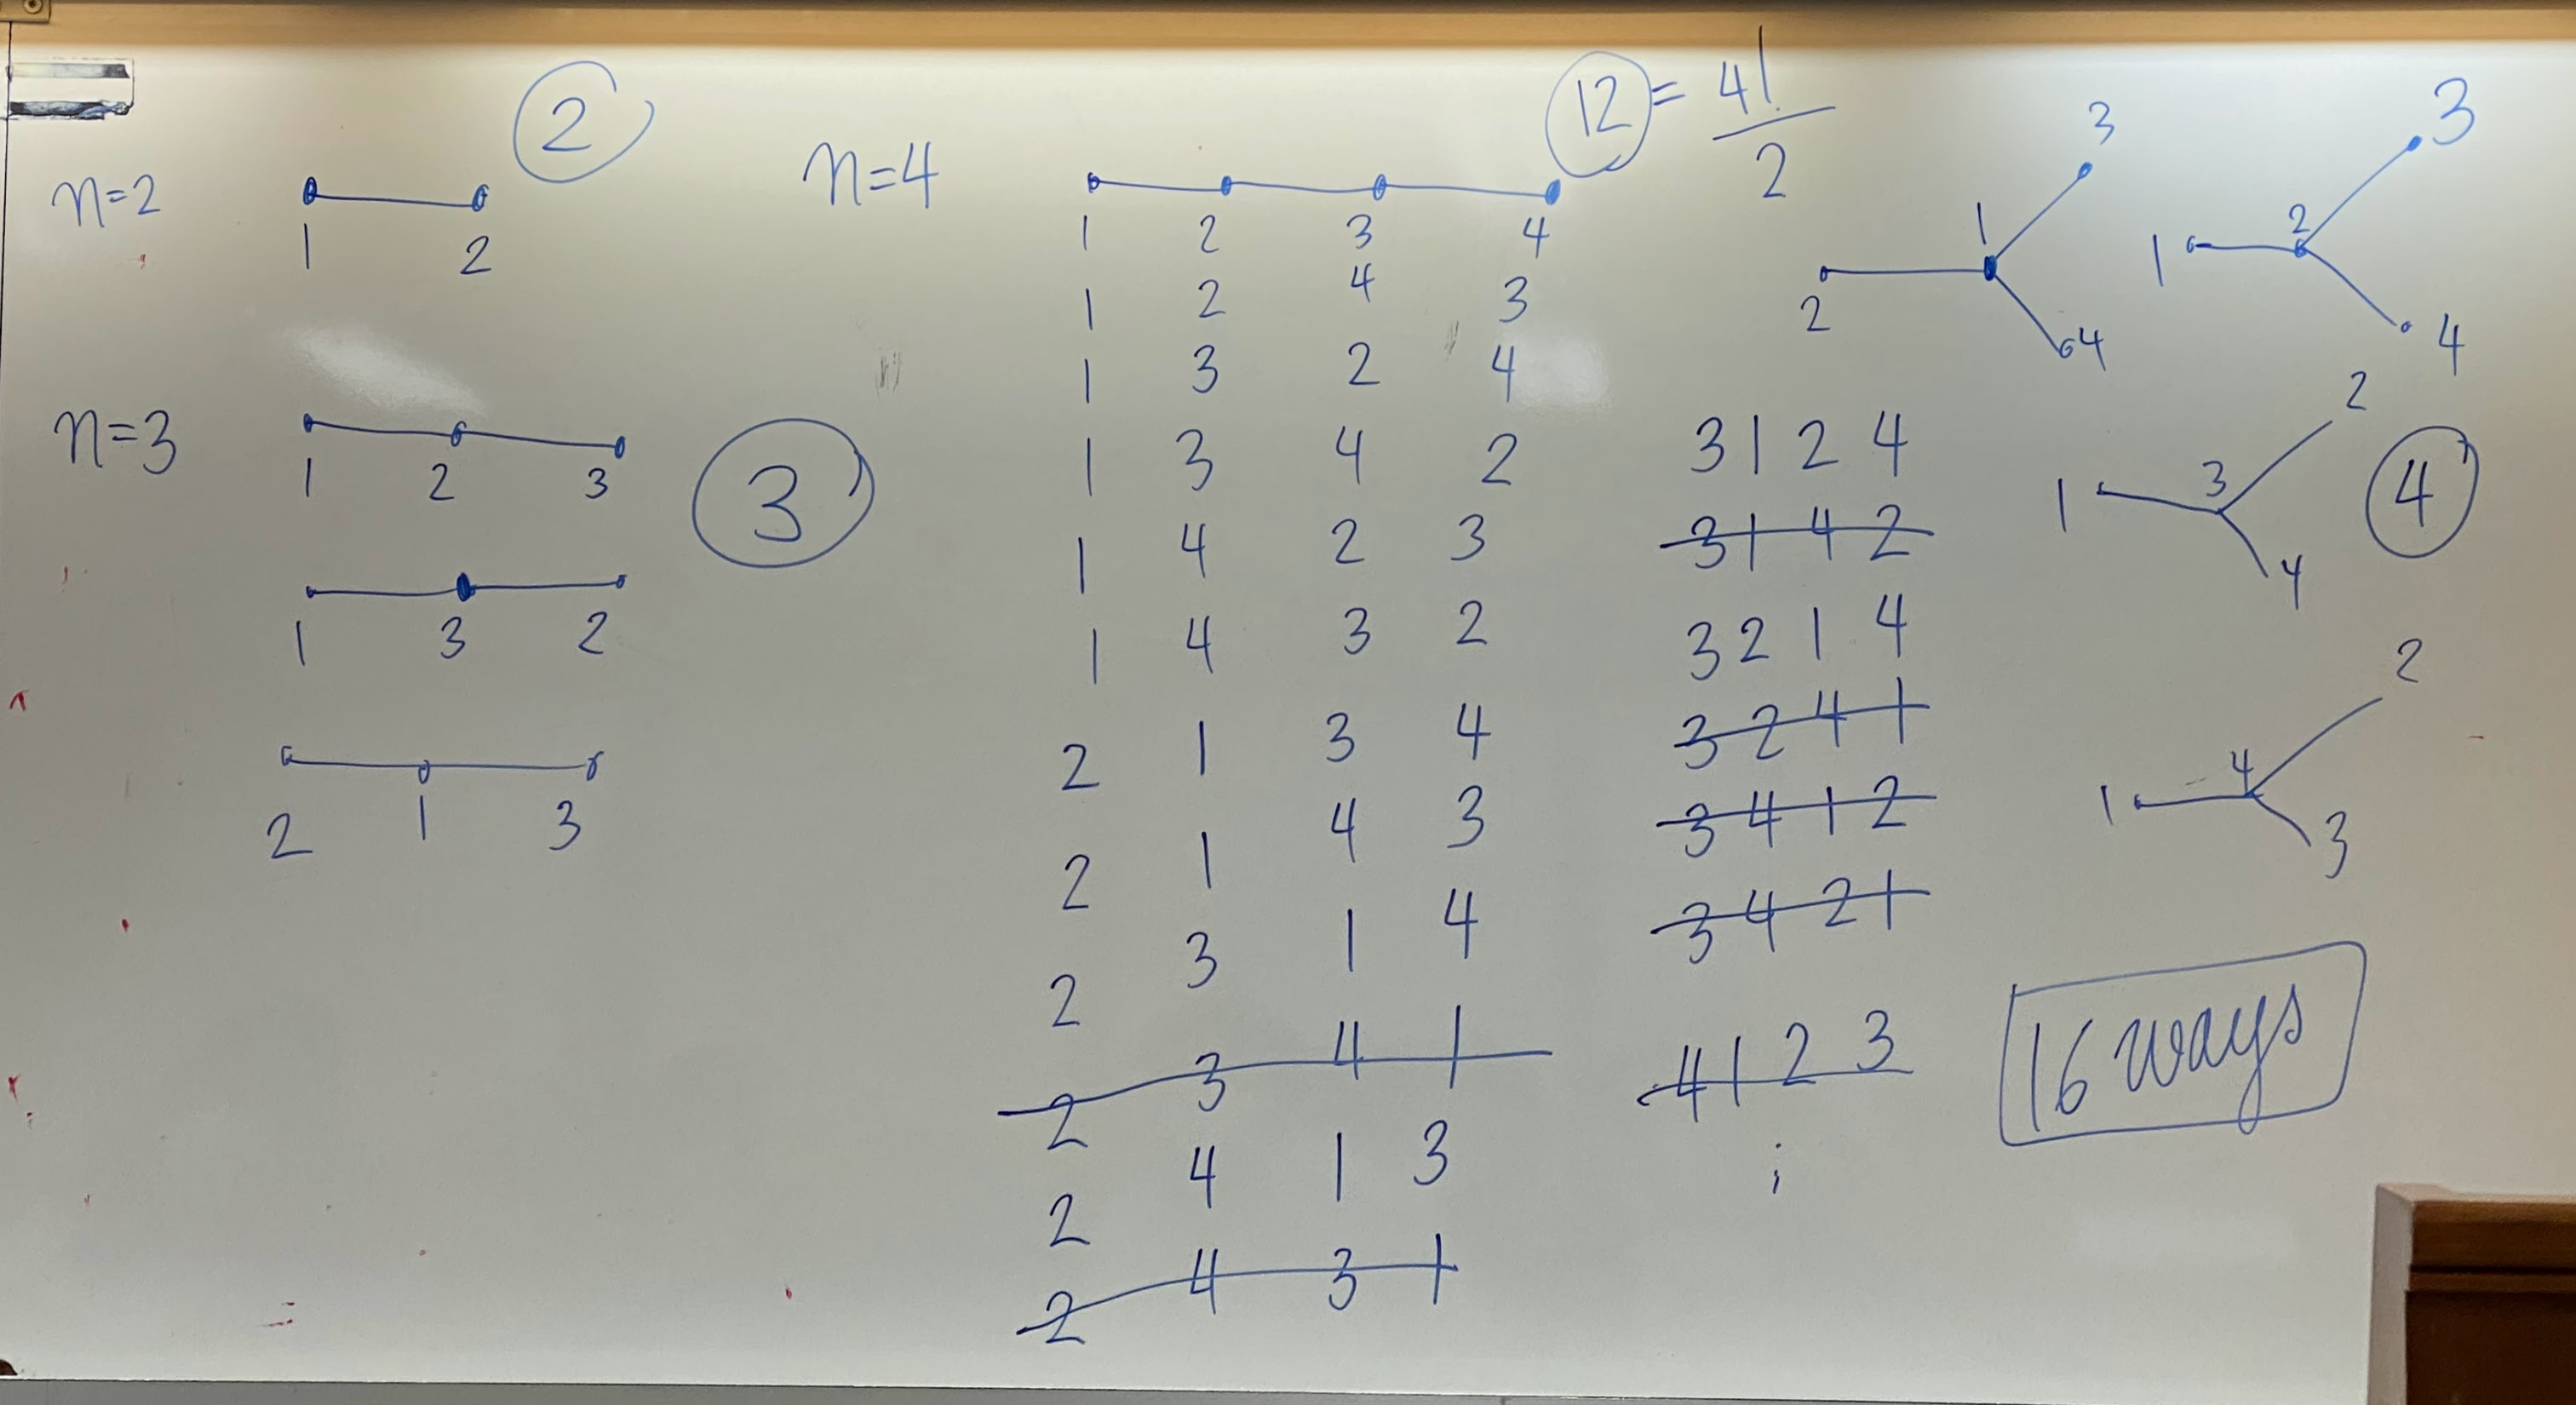
\includegraphics[width=0.95\textwidth]{figures/l05/label1}

    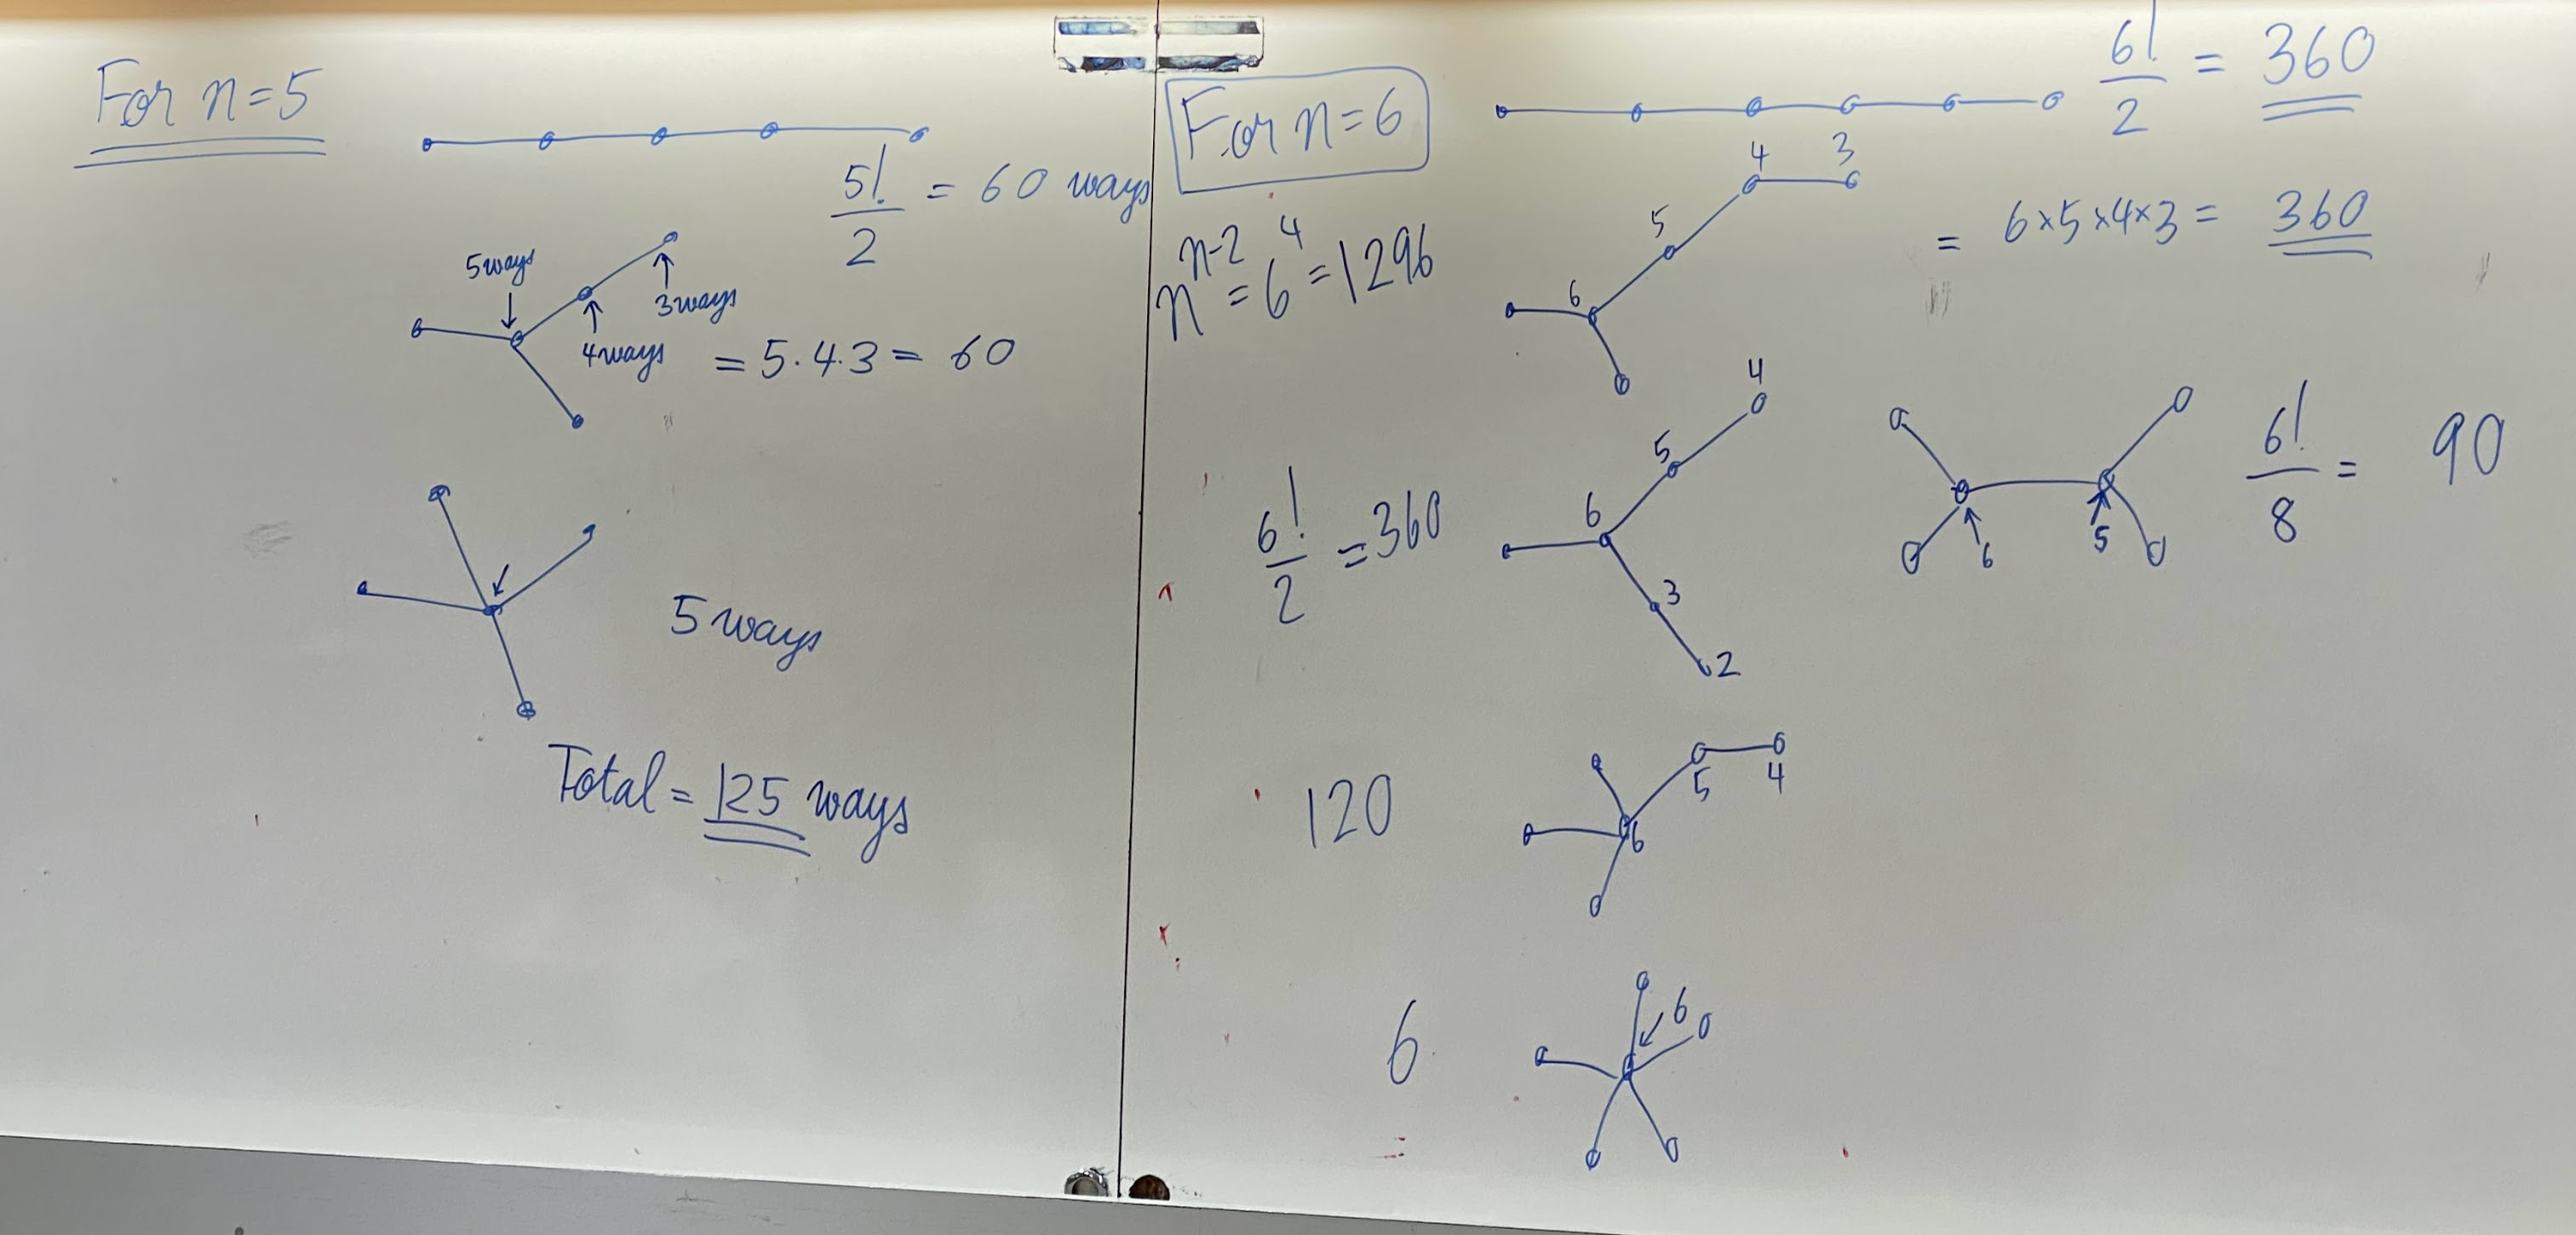
\includegraphics[width=0.95\textwidth]{figures/l05/label2}
  \end{center}
  \caption{Examples of labelled trees for \(n=2,3,4,5,6\)}\label{fig:label-examples}
\end{nexample}
\end{figure}
